\documentclass[12pt,letterpaper]{article}
\usepackage[utf8]{inputenc}
\usepackage[spanish]{babel}
\usepackage{amsmath}
\usepackage{amsfonts}
\usepackage{amssymb}
\usepackage{natbib}
\usepackage{graphicx}
\usepackage{cite}
\usepackage{wrapfig}
\usepackage{afterpage}
\setcitestyle{square}
\usepackage[export]{adjustbox}
\usepackage[left=2cm,right=2cm,top=2cm,bottom=2cm]{geometry}
\usepackage{afterpage}
\usepackage{setspace}
\spanishdecimal{.}
\usepackage{hyperref}
\usepackage{float}

\author{C. Iván Pineda S.\textsuperscript{1} }
\title{Implementación de un algoritmo evolutivo para determinar orbitas en un modelo del sistema solar\\ IIMAS}
\date {\textit{\textsuperscript{1}Universidad Nacional Autónoma de México}
\\ 5 de junio de 2018}

\begin{document}
\maketitle

\begin{abstract}
El objetivo de este trabajo es modelar el sistema solar y su dinámica utilizando las ecuaciones de movimiento para un sitema de dos cuerpos en el caso de la interacción planeta-estrella y un sistema de n-cuerpos para el caso de la nave, además, se empleó un algoritmo genético para encontrar las trayectorias óptimas para el viaje desde la Tierra hasta otro cuerpo del sistema solar, la función de evaluación de dicho algoritmo recibe la velocidad inicial de la nave y el tiempo inicial al despegar, utiliza el método de Euler para resolver las trayectorias de cada uno de los cuerpos y regresa la distancia mínima a la que estuvo la nave y el planeta destino, además, se anexa una animación para visualizar los resultados.
\end{abstract}


\section*{Introducción}

\subsection*{Mecánica newtoniana}

La interacción gravitatoria no relativista de dos cuerpos con masa se describe básicamente con la segunda ley de Newton y con la ley de gravitación universal \citep{jose2000classical}.

\begin{equation}
 M\dfrac{d ^2 \mathbf{r_2}}{d t^2}=-G\dfrac{m_1m_2}{|\mathbf{r_{2}}-\mathbf{r_1}|^3}(\mathbf{r_{2}}-\mathbf{r_1})
\end{equation} 

Donde:
\\
\\
$M=\dfrac{m_1m_2}{m_1+m_2}$, es el centro de masas del sistema.
\\
\\
$G=39.4784176 \ AU^3 \ YR^{-2} \ SM^{-1}$, G es la constante de gravitación universal, AU=Unidad Astronómica, YR=Año, SM=Masas solares.
\\
\\
$\mathbf{r_n} $ es el vector de posición de cada cuerpo.
\\
\\
Como la masa del Sol comparada con la de los planetas es varios ordenes de magnitud mayor, podemos decir que $m_s>>m_p$, por lo tanto:
\\
\\
$M=\dfrac{m_sm_p}{m_s+m_p}=\dfrac{m_sm_p}{m_s}=m_p$, sustituyendo en la ecuación (1).

\begin{equation}
 m_p\dfrac{d ^2 \mathbf{r_p}}{d t^2}=-G\dfrac{m_sm_p}{|\mathbf{r_{p}}-\mathbf{r_s}|^3}(\mathbf{r_{p}}-\mathbf{r_s}) \Rightarrow \dfrac{d ^2 \mathbf{r_p}}{d t^2}=-G\dfrac{m_s}{|\mathbf{r_{p}}-\mathbf{r_s}|^3}(\mathbf{r_{p}}-\mathbf{r_s})
\end{equation} 

La ecuación (2) determina la dinámica de un planeta con respecto al Sol, para determinar la dinámica de la nave debemos sumar las fuerzas de cada uno de los planetas y del Sol, basándonos en lo que realizamos para obtener la ecuación (2) pero ahora siendo $m_{planetas}>>m_{nave}$ obtenemos:

\begin{equation}
\dfrac{d ^2 \mathbf{r_{nave}}}{d t^2}=\sum_{i=1}^{9} -G\dfrac{m_i}{|\mathbf{r_{nave}}-\mathbf{r_i}|^3}(\mathbf{r_{nave}}-\mathbf{r_i})=-G \sum_{i=1}^{9} m_ i\dfrac{\mathbf{r_{nave}}-\mathbf{r_i}}{|\mathbf{r_{nave}}-\mathbf{r_i}|^3}
\end{equation}

Donde $m_i$ y $r_i$ representan la masa y posición de cada uno de los planetas y el Sol.

Para obtener la velocidad debemos integrar las ecuaciones (2) y (3).
\begin{equation}
\mathbf{v_{planeta}}\equiv\int_{0}^{t} \dfrac{d ^2 \mathbf{r_p}}{d t^2} dt=-G \int_{0}^{t} \dfrac{m_s}{|\mathbf{r_{p}}-\mathbf{r_s}|^3}(\mathbf{r_{p}}-\mathbf{r_s}) dt
\end{equation}

\begin{equation}
\mathbf{v_{nave}}\equiv\int_{0}^{t} \dfrac{d ^2 \mathbf{r_{nave}}}{d t^2} dt=-G \int_{0}^{t} \sum_{i=1}^{9} m_ i\dfrac{\mathbf{r_{nave}}-\mathbf{r_i}}{|\mathbf{r_{nave}}-\mathbf{r_i}|^3} dt
\end{equation}

Como el objetivo del curso es usar métodos numéricos, vamos a obtener cada punto siguiente utilizando el método de Euler, entonces la forma en que vamos a utilizar las ecuaciones (4) y (5) es:
\begin{equation}
\mathbf{v_{planeta_{t+1}}}=\mathbf{v_{planeta_t}}-G\dfrac{m_s}{|\mathbf{r_{p_t}}-\mathbf{r_{s_t}}|^3}(\mathbf{r_{p_t}}-\mathbf{r_{s_t}})dt
\end{equation}

\begin{equation}
\mathbf{v_{nave_{t+1}}}=\mathbf{v_{nave_t}}-G \sum_{i=1}^{9} m_ i\dfrac{\mathbf{r_{nave_t}}-\mathbf{r_{i_t}}}{|\mathbf{r_{nave_t}}-\mathbf{r_{i_t}}|^3}dt
\end{equation}

Para obtener la posición actual en función de la posición anterior utilizamos la ecuación de posición para un movimiento uniformemente acelerado que se obtiene al integrar dos veces con respecto al tiempo las ecuaciones (2) y (3), suponiendo que la distancia que separa a los cuerpos no varia significativamente del punto anterior al punto siguiente si usamos un $dt$ pequeño, por lo que la aceleración se puede tomar como constante, entonces:

\[
\mathbf{a} \equiv -G \sum_{i=1}^{9} m_ i\dfrac{\mathbf{r_{nave}}-\mathbf{r_i}}{|\mathbf{r_{nave}}-\mathbf{r_i}|^3} \approx cte
\]

Por lo tanto la velocidad es:

\begin{equation}
\mathbf{v_{nave}}\equiv \dfrac{d  \mathbf{r_{nave}}}{d t} \equiv \int_{0}^{t} \dfrac{d ^2 \mathbf{r_{nave}}}{d t^2} dt= \int_{0}^{t} \mathbf{a} dt
\end{equation}

Resolviendo la ecuación (8):

\[
\dfrac{d  \mathbf{r_{nave}}}{d t} \mid_{0}^{t}= \mathbf{a}t \mid_{0}^{t} \ \Rightarrow \mathbf{v_{nave}}(t)-\mathbf{v_{nave}}(0) = \mathbf{a}t - \mathbf{a}0
\]

Tomando a $\mathbf{v_{nave}}(0)=\mathbf{v_{nave_0}}=cte$, tenemos que:

\begin{equation}
\mathbf{v_{nave}}(t)=\mathbf{v_{nave_0}} + \mathbf{a}t
\end{equation}

La ecuación (9) también se puede escribir de la forma $\dfrac{d  \mathbf{r_{nave}}(t)}{d t}=\mathbf{v_{nave_0}} + \mathbf{a}t$, la integral de dicha ecuación con respecto al tiempo nos dará la ecuación de movimiento para la nave.

\begin{equation}
 \int_{0}^{t} \dfrac{d  \mathbf{r_{nave}}(t)}{d t} dt= \int_{0}^{t} [\mathbf{v_{nave_0}} + \mathbf{a}t] dt
\end{equation}

Resolviendo la ecuación (10):

\[
\mathbf{r_{nave}}(t) \mid_{0}^{t} = [\mathbf{v_{nave_0}}t + \dfrac{1}{2}\mathbf{a}t^2] \mid_{0}^{t} \ \Rightarrow \ 
\mathbf{r_{nave}}(t) - \mathbf{r_{nave}}(0) = [\mathbf{v_{nave_0}}t + \dfrac{1}{2}\mathbf{a}t^2] - [\mathbf{v_{nave_0}}0 + \dfrac{1}{2}\mathbf{a}0^2]
\]

Tomando a $\mathbf{r_{nave}}(0)=\mathbf{r_{nave_0}}=cte$ y remplazando a $\mathbf{a}$ tenemos que la ecuación de movimiento para la nave es:

\begin{equation}
\mathbf{r_{nave}}(t) = \mathbf{r_{nave_0}} + \mathbf{v_{nave_0}}t - \dfrac{1}{2}\ G \sum_{i=1}^{9} m_ i\dfrac{\mathbf{r_{nave}}-\mathbf{r_i}}{|\mathbf{r_{nave}}-\mathbf{r_i}|^3} t^2
\end{equation}

Realizando un procedimiento similar, la ecuación de movimiento para cada uno de los planetas es:

\begin{equation}
\mathbf{r_{p}}(t) = \mathbf{r_{p_0}} + \mathbf{v_{p_0}}t - \dfrac{1}{2}\ G\dfrac{m_s}{|\mathbf{r_{p}}-\mathbf{r_s}|^3}(\mathbf{r_{p}}-\mathbf{r_s}) t^2
\end{equation}

La resolución numérica de dichas ecuaciones para cada iteración es:

\begin{equation}
\mathbf{r_{nave_{t+1}}} = \mathbf{r_{nave_t}} + \mathbf{v_{nave_t}}dt - \dfrac{1}{2}\ G \sum_{i=1}^{9} m_ {i}\dfrac{\mathbf{r_{nave_t}}-\mathbf{r_{i_t}}}{|\mathbf{r_{nave_t}}-\mathbf{r_{i_t}}|^3} dt^2
\end{equation}

\begin{equation}
\mathbf{r_{p_{t+1}}} = \mathbf{r_{p_t}} + \mathbf{v_{p_t}}dt - \dfrac{1}{2}\ G\dfrac{m_s}{|\mathbf{r_{p_t}}-\mathbf{r_{s_t}}|^3}(\mathbf{r_{p_t}}-\mathbf{r_{s_t}}) dt^2
\end{equation}

Para modelar la dinámica de nuestro sistema solo usaremos las ecuaciones (6), (7), (13) y (14), las condiciones iniciales que se asignaran al algoritmo genético son $t_0$, $v_{x_0}$, $v_{y_0}$, mientras que $\mathbf{r}=(x(t),y(t),z(t))$, $\mathbf{v}=(v_x(t),v_y(t),v_z(t))$, $z(t)=0$ y $v_z(t)=0$ para todo t.

\subsection*{Algoritmos genéticos}

Los algoritmos genéticos son un método heurístico de optimización que se utiliza para encontrar los máximos y mínimos de una función sin necesidad de usar derivadas, se basan en la selección natural \citep{gestal2010introduccion}.

\subsubsection*{Codificación binaria}

En la naturaleza la información necesaria para codificar las proteínas que constituyen a los seres vivos está almacenada en una cadena de ADN, dicha cadena se compone de solo 4 bases; adenina, guanina, citosina y timina, posteriormente se realiza una transcripción a ARN que se compone de las mismas bases, solo se cambia timina por uracilo y finalmente se realiza la traducción a proteínas. 

Para nuestro algoritmo utilizaremos una codificación en números binarios, es decir, una cadena de solo 0 y 1 que posteriormente será traducida a un número decimal que se encuentre dentro de un intervalo dado.

En un inicio se crearán un número determinado de cadenas de binarios que será nuestra población, que tendrán un número determinado de bits al que llamaremos $n$ y la distribución de 0 y 1 será aleatoria.

Primero convertimos la cadena binaria a decimal como en el siguiente ejemplo:

\[
dec=101011_2=1*2^5+0*2^4+1*2^3+0*2^2+1*2^1+1*2^0=32+0+8+0+2+1=43
\]

Posteriormente para tener el decimal en el intervalo en el que vamos a evaluar a nuestra función utilizamos:

\begin{equation}
decInt=a+\dfrac{dec}{2^n-1}(b-a)
\end{equation}

Donde $a$ y $b$ son el inicio y final de nuestro intervalo, $n$ es el número de bits de nuestra cadena y $dec$ es nuestra primer conversión de binario a decimal, $decInt$ es el decimal que recibe la función de evaluación.

\subsubsection*{Selección}

Si buscamos encontrar los mínimos seleccionaremos aquellas cadenas que al ser convertidas a decimal y al evaluarlas en nuestra función $f(v_{x_0},v_{y_0},t_0)$ nos den resultados más pequeños, es decir, las cadenas que produzcan las trayectorias más cercanas al planeta destino, nuestra función evidentemente tiene un gran número de mínimos, obtenerlos con métodos numéricos o analíticos convencionales no es lo más efectivo.

El punto $P$ es un mínimo local de $f$ si existe un entorno reducido de centro $x_0$, que cumpla que $f(x)\geq f(x_0) \ \forall x \in E'(x_0)$. $P(x_0,f(x_0))$ es un mínimo absoluto de $ f \Longleftrightarrow \forall x \neq x_0, A, f(x_0)\leqslant f(x)$, donde $A$ es un subconjunto del dominio de $f$.

La cantidad de cadenas a seleccionar puede variar, para este trabajo se utilizó la mitad de la población, es decir solo el 50\% más adaptado podrá reproducirse.

\subsubsection*{Reproducción}

Una vez que se seleccionaron los individuos más aptos, dejarán su descendencia, se seleccionan dos cadenas al azar y apartir de ellas se crea una cadena hija, para este algoritmo se genera una cantidad de cadenas hijas igual a la cantidad de cadenas padres, es decir, la mitad de la población inicial, así padres e hijos sumaran la misma cantidad de cadenas que al inicio.

Hay varias formas de combinar los genes (unidades de información, en este caso bits), aquí se utilizó el cruce uniforme que consiste en formar una cadena hija a partir de dos padres, donde cada bit de las cadenas padres tiene un 50 \% de probabilidad de pasar al hijo. Esto se logra seleccionando aleatoriamiente un bit en una posición específica de las cadenas padres (lo más fácil es empezar en la posición 0 y terminar en el último carácter de la cadena), dicho bit se asigna en la misma posición para el hijo y se descarta esa posición.

\subsubsection*{Mutación}

Las mutaciones son esenciales para mantener la variabilidad en nuestra población, sin estas, nuestros individuos tendrán el mismo valor en un menor número de generaciones, esto es ideal sí ese valor corresponde a un mínimo, pero casi nunca es así.

Para mutar a un individuo es necesario cambiar aleatoriamente el valor de algunos de sus genes o bits, para esto se genera un número aleatorio en un intervalo que va desde el 0 hasta la longitud de la cadena menos 1, se escoge la posición en la cadena correspondiente a ese número y se intercambia su valor por 0 si era 1 y viceversa, se realiza lo mismo el número de veces que se quiera mutar al individuo.

\subsubsection*{Algoritmo principal}

Los pasos que se llevan a cabo son los siguientes:

\ \ \ \ \ 1. Generación de una población inicial de cadenas.

\ \ \ \ \ 2. Selección de las más aptas.

\ \ \ \ \ 3. Reproducción.

\ \ \ \ \ 4. Mutación solo en los hijos.

\ \ \ \ \ 5. Generación de una nueva población que es la suma de los padres y los hijos.

\ \ \ \ \ 6. Se regresa al paso 2 con la generación obtenida en el paso 5 hasta una condición de paro 

\ \ \ \ \ \ \ \ o cuando se alcance el número especificado de iteraciones.

\ \ \ \ \ 7. Se imprimen o guardan los valores de la última generación.

\section*{Métodos}

Nos basamos en un artículo sobre el Diseño de un programa en python para la enseñanza de la transferencia de
órbita de Hohmann \citep{mendez2016diseno}.

Se utilizó python para la elaboración de los algoritmos, la libreria de math y numpy para el desarrollo matemático, random para generar números aleatorios y Visual Python para el modelo visual, el código se puede revisar en \url{https://github.com/Ivan252512/TallerDeModelacion/tree/master/Exposicion}. Visual python es la única que no se instala con Anaconda, para hacerlo es necesario ejecutar desde la terminal de Linux \textbf{pip install vpython}, para más información visitar el sitio \url{http://vpython.org}.

Para todos los destinos los datos de entrada para $v_x$ y $v_y$ fueron asignados dentro del intervalo [-7.5 UA/YR, 7.5 UA/YR] o [-128 000 km/hr, 128 000 km/hr], las iteraciones necesarias para encontrar trayectorias que lleguen al destino son menores  para los planetas interiores, para Urano y Neptuno el programa tardó días en terminar, mientras que para Marte tarda solo unos minutos. El tiempo al que iniciaba el viaje también dependía del destino.

Además, si $|v_{nave}|\equiv \sqrt{v_x^2+v_y^2+v_z^2}>7.5$ UA/YR con $v_z=0$, la función regresa 5000 UA, esto para evitar trayectorias donde la nave tuviera una rápidez mayor a la del límite propuesto para la simulación, dicho límite 
es la rápidez tangencial de la Tierra más 21 000 km/hr del cohete, esta rápidez es alcanzable por los cohetes actuales, aunque para las condiciones de despegue no se tomó en cuenta la velocidad relativa entre el cohete y la Tierra, más bien el cohete despega de un punto con las coordenadas de la Tierra, pero se ignora que en primer instancia está viajando a bordo de dicho planeta, es una consideración a tomar en cuenta para mejorar la simulación.

Si la trayectoria del cohete pasa a menos de 0.5 UA del sol, la función regresa 10 000 UA, esto se delimitó debido a que trayectorias tan cercanas al Sol pueden averiar la nave, además, el algoritmo sin esa restricción tendía a regresar órbitas que usaban al Sol como un acelerador debido a su gran masa, siempre pasando muy creca de la estrella.

Cuando en algún punto de toda la trayectoria la nave pasaba a menos de $|\mathbf{r_{destino}}-\mathbf{r_{nave}}|-0.1$ UA de su destino, el algoritmo ordenaba una lista de todas sus posiciones y regresaba el valor con la distancia más pequeña.

Si la nave pasaba a menos de 0.05 UA de su destino, el primer valor que cumpliera dicha condición es el que se regresaba y si ninguna de todas estas condiciones se cumplia, se regresaba el último valor de la distancia entre la nave y el destino.

\section*{Resultados}

\subsection*{Marte}

El tiempo de inicio estaba dentro del intervalo de [0,2 500] con 10 000 iteraciones por individuo, los tres parametros tenían 100 individuos de 20 bits cada uno y el algoritmo genético se corrió para 25 generaciones, el mejor valor fue en (fig. \ref{fig:marte}):

\[
f(6.8707317073170735, 0.6998998641012797, 1096.0) = 0.04745463993063615
\]


\begin{figure}[H]
\centering
  \begin{minipage}{0.3\textwidth}
    \centering
    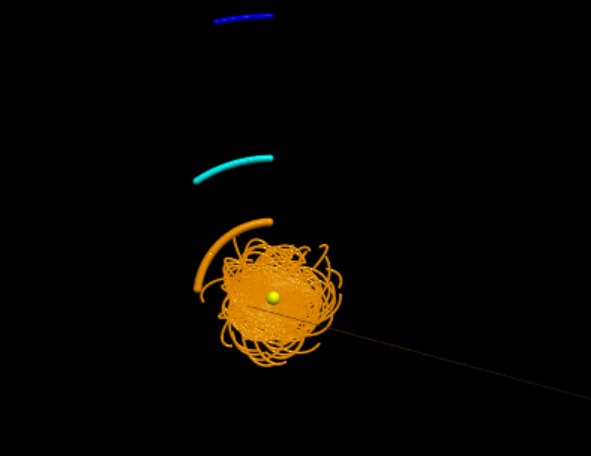
\includegraphics[width=0.885\textwidth]{marte}\\
    {\small (a)} 
  \end{minipage}%
  \hspace{1mm}
  \begin{minipage}{0.3\textwidth}
    \centering
    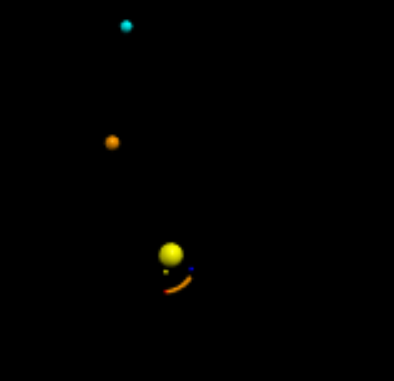
\includegraphics[width=0.8\textwidth]{marteop}\\
    {\small (b)} 
  \end{minipage}
  \caption{Marte: (a) Trayectorias generadas aleatoriamente. (b) Mejor trayectoria.}
  \label{fig:marte}
\end{figure}


\subsection*{Júpiter}

El tiempo de inicio estaba dentro del intervalo de [0,50 000] con 100 000 iteraciones por individuo, los tres parametros tenían 50 individuos de 20 bits cada uno y el algoritmo genético se corrió para 25 generaciones, el mejor valor fue en (fig. \ref{fig:jupiter}):

\[
f(-4.232908947857807, 6.565088334167799 29406, 0.04981131056035353) = 0.04981131056035353
\]

\begin{figure}[H]
\centering
  \begin{minipage}{0.3\textwidth}
    \centering
    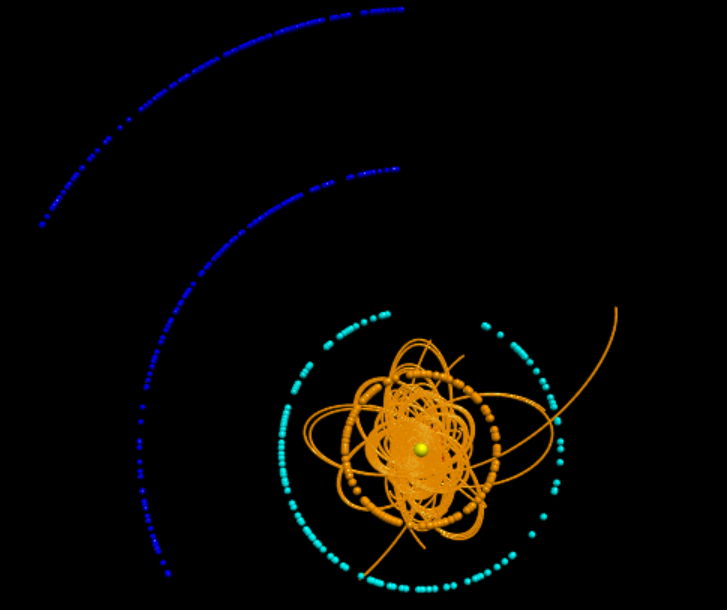
\includegraphics[width=0.885\textwidth]{Jupiter}\\
    {\small (a)} 
  \end{minipage}%
  \hspace{1mm}
  \begin{minipage}{0.3\textwidth}
    \centering
    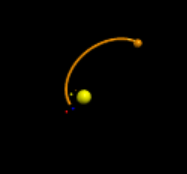
\includegraphics[width=0.8\textwidth]{JupiterFinal}\\
    {\small (b)} 
  \end{minipage}
  \caption{Júpiter: (a) Trayectorias generadas aleatoriamente. (b) Mejor trayectoria.}
  \label{fig:jupiter}
\end{figure}

\section*{Conclusiones}

El algoritmo genético resultó efectivo y encontramos trayectorias que llevaban a la nave a su destino, aun queda mucho por mejorar en el modelo, principalmente agregar a la nave una velocidad inicial que también tome en cuenta la velocidad de traslación y rotación de la Tierra, tomar en cuentas los momentos angulares y posibles torcas del sistema y ya si se quiere ser mucho más específico más cuerpos celestes y la interacción con el viento solar.

En definitiva, la simulación tiene más potencial.


\bibliography{TrabajoFinal}
\bibliographystyle{apa}

\end{document}

